

\begin{flushleft}
	\begin{itemize}
		\item Least frequently used data type.
		\item short keyword is 16-bit signed integer. 
		
		\tabletwo{
		\hline
		Size & \textbf{2 byte (16 bits)} \\
		\hline
		MAX\_VALUE & 32767 \\
		\hline
		MIN\_VALUE & -32768 \\
		\hline
		Range & \textbf{-$2^\textbf{15}$} to \textbf{$2^\textbf{15}$-1}  \\
		\hline
		}
		\bigskip
		\item \textbf{Where is short data type used?}
		\begin{itemize}
			\item Short data type used for 16 bit processor like 8085.
		\end{itemize}	
	
		\begin{figure}[h!]
			\centering
			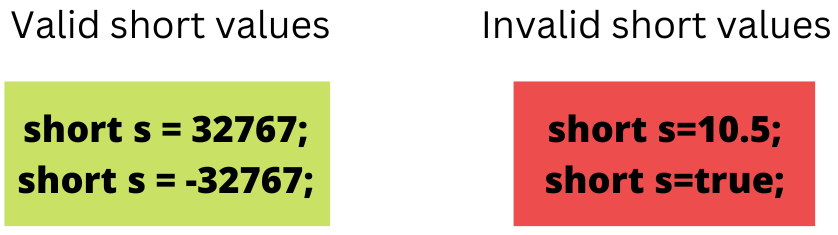
\includegraphics[scale=.38]{content/chapter2/images/short.png}
		\end{figure}		
	\end{itemize}
	
\end{flushleft}

